\section{Program Modelling}
When translating a program to a UPPAAL model, several approaches are possible, depending on what is to be shown. One could for example represent a program merely in terms of program flow, if a disruption of program flow is to be simulated, e.g an error in the program counter. A memory corruption could be simulated by including the data flow in the model. These are just a few examples and many representations can be chosen. We have chosen the latter and model programs in terms of program and data flow to simulate disruptions in the execution flow.
%
\subsection{Program Conversion}\label{sec:programConversion}
The program conversion is based on \jcl semantics, most Java bytecode instructions can be translated directly to \jcl, but type information is lost. Because \jcl has operational semantics defined, it eases the implementation of the simulation, since each instruction is clearly defined.\\\\
A Java method is represented by a template and method invocation is done by channels. This representation restricts the possibilities of recursion, and additionally the maximum memory usage must be known for allocation purposes. 
These limitations, while very restrictive for general Java, are already considered good practice for Java Card programming due the limited hardware, as discussed in \cref{subsec:smartcard}.
A program instruction, such as \texttt{ALOAD a} and \texttt{DUP} are represented as UPPAAL locations, this implies that a change in the program counter results in a change of location. 
In turn, this means that when an instruction is executed, the change to the program configuration \textit{Conf} from \cref{sec:semintro} occurs on the edge to the next location.


\begin{lstlisting}[caption={Java code sample to be converted to a UPPAAL model.}, label={lst:ternary}]
public class Sample{
    public class Sample{
        public static void main(String[] args) {
            install();
            foo(3);
        }
        
        public static int foo(int i){
            return i != 0 ? 1 : 2;
        }
    }
}
\end{lstlisting}

\begin{figure}
\begin{subfigure}{\textwidth}
	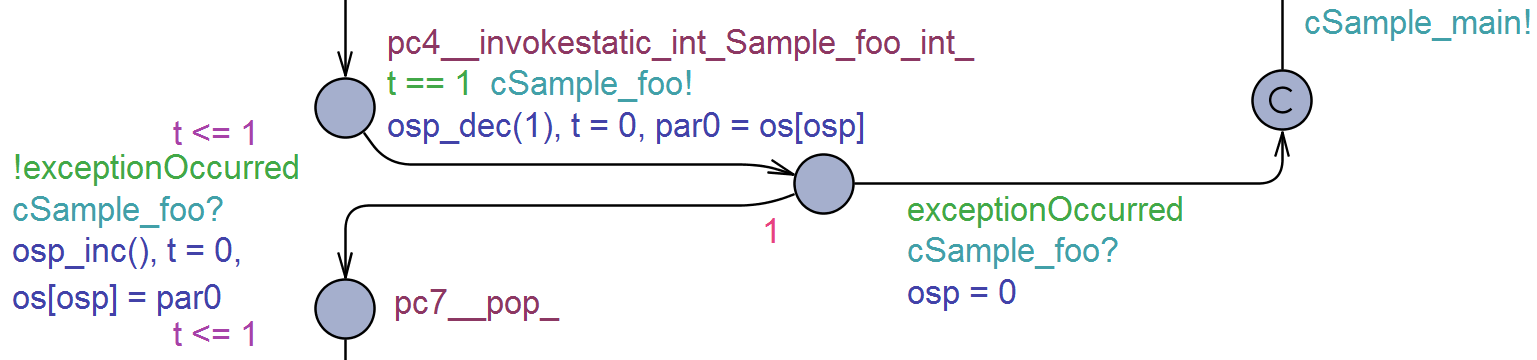
\includegraphics[width=\textwidth]{invokefoo.PNG}
	\caption{Method call in \texttt{main}.}
\end{subfigure}
\begin{subfigure}{\textwidth}
	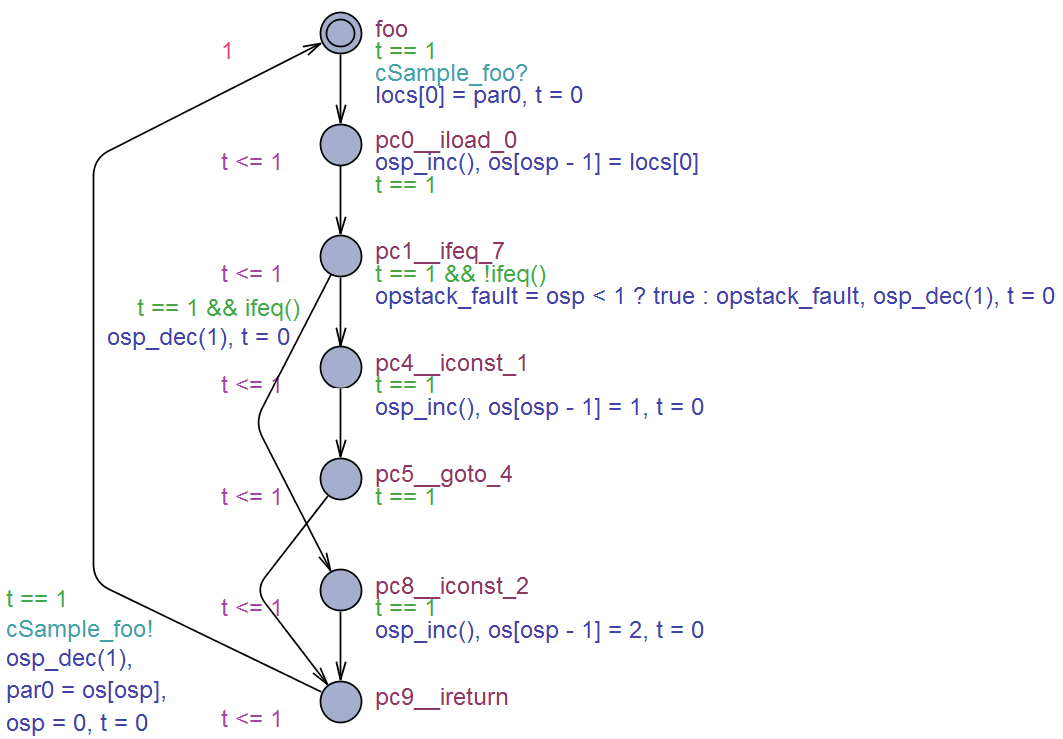
\includegraphics[width=\textwidth]{foomethod.PNG}
	\caption{the method \texttt{foo}.}
	\label{fig:uppaal3}
\end{subfigure}

\caption{Auto generated model of the \texttt{foo} method from \cref{lst:ternary}}
\label{fig:fooMethod}
\end{figure}


\subsubsection{Simple Instructions}
\begin{figure}[H]
\centering
\begin{subfigure}{.3\textwidth}
  \begin{lstlisting}[numbers=none]
0. iload 0
1. ifeq 7
...
  \end{lstlisting}
  \caption{Java Bytecode Sample.}
\end{subfigure} 
\hspace{10px}
\begin{subfigure}{.6\textwidth}
  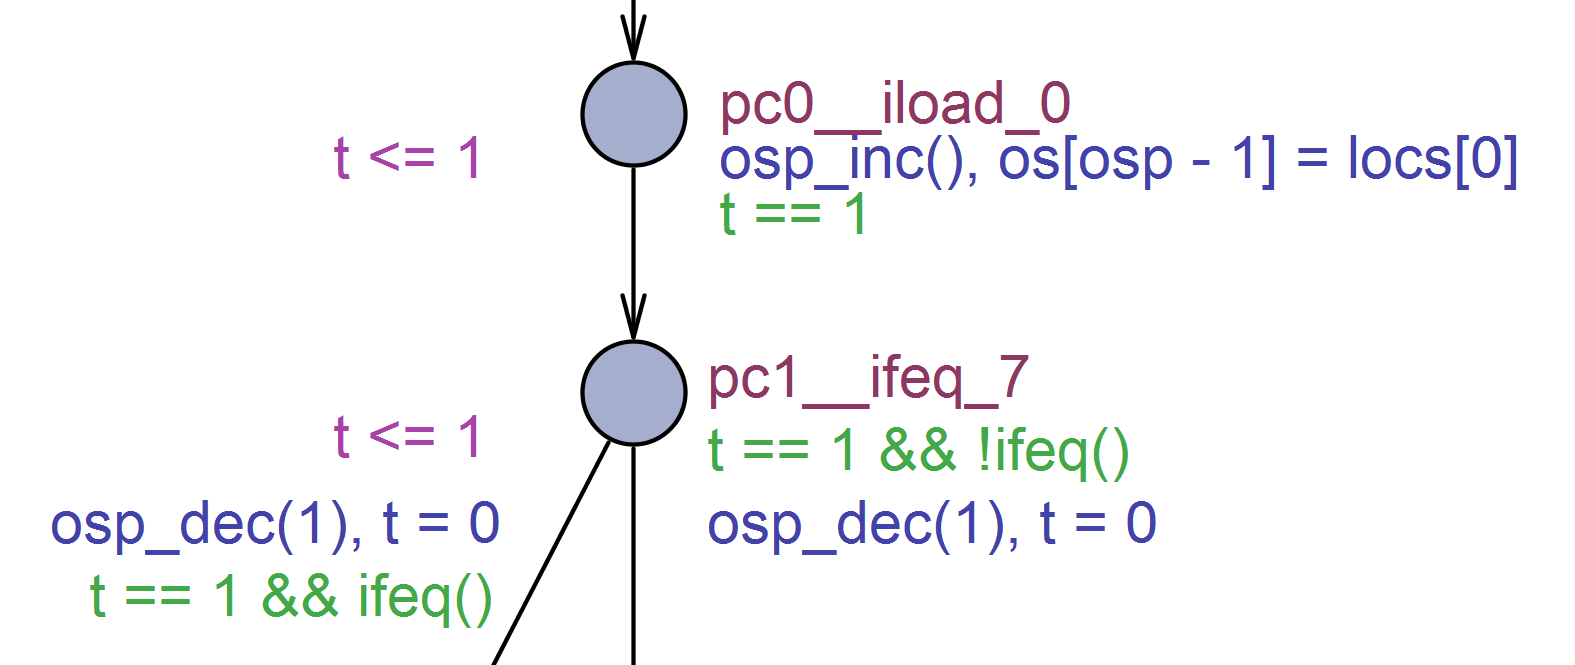
\includegraphics[width=\textwidth]{ifeq.PNG}
  \caption{Generated model from Sample.}
\end{subfigure}
\caption{Java bytecode and corresponding UPPAAL model.}
\label{fig:uppaal1}
\end{figure}

\Cref{fig:uppaal1} shows how two Java bytecode instructions are represented in UPPAAL. On the left we see the Java bytecode. In the first line with pc 0, we have the \texttt{iload 0} instruction. \texttt{iload 0} pushes an integer from local variables at position zero on top of the operand stack, and increments the operand stack pointer and program counter.
In UPPAAL the location \UPP{pc0\_iload\_0} represents \texttt{iload 0}. The UPPAAL model is seen in \Cref{fig:uppaal1}b.\\\\
% %
We have decided each non-library instruction to take $1$ time unit, this is simulated with the location invariant \UPP{t <= 1} and guard \UPP{t == 1} on the edge leading to the next location. The guard is found below the location name, right of the edge and invariant is to the left of the edge. In this sample we defined the execution time as 1 time unit.\\\\
In the update on the edge seen below the guard, we simulate the data flow by assigning the value of the local variable, \UPP{locs\relax[0\relax]}, to the element at the top of the operand stack, \UPP{os}, represented by operand stack pointer, \UPP{osp}. \UPP{osp} is incremented as the operand stack grows and the increment of the program counter is simulated by the edge itself.

\subsubsection{Jumps and Branches}
For the majority of instructions the program counter is set to the next instruction after execution, but for a jump with \texttt{goto a} the edge goes to the instruction with the program counter corresponding to the value of \texttt{a}, as seen in \Cref{fig:fooMethod}.\\\\
% %
Conditionals such as \texttt{if\_cmpeq a} are modelled by a location having two outgoing edges, see \Cref{fig:uppaal1}, one to the next instruction and one to a the location with a program counter with an offset of \texttt{a}. On these edges, the guard is used to determine which of the edges is to be traversed.

\subsubsection{The Operand Stack, Local Variables and the Heap}
To simulate the operand stack, we use an operand stack pointer to point at the next free position in an array. Local variables and the heap are both represented as arrays in the UPPAAL model, but they do not use an explicit pointer to access them since access to these are not necessarily performed in a top-down manner as with the operand stack.

\subsubsection{Method Calls}\label{subsubsec:method}
Method calls cover the Java bytecode instructions: \texttt{invokestatic} for static calls, \texttt{invokespecial} for class constructors and private calls, and \texttt{invokevirtual} for virtual calls. To illustrate how these instructions are modelled, we use the Java code sample in \cref{lst:virtual}.
\begin{lstlisting}[caption={\texttt{Bclass} extends \texttt{Aclass}, \texttt{Aclass} implements the methods foo and bar, and \texttt{Bclass} overwrites foo.}, label={lst:virtual}]
public class Virtual{
  public Aclass a;
  public Aclass b;

  public Virtual(){
    a = new Aclass();
    b = new Bclass();
    int ia = a.foo() + a.bar();
    int ib = b.foo() + b.bar();
  }
}
\end{lstlisting}
The sample includes the bytecode instructions \texttt{invokespecial} and \texttt{invokevirtual}.
\texttt{invokestatic} are omitted as \texttt{invokestatic} and \texttt{invokespecial} are nearly identical, the only difference being whether an object reference from the operand stack is passed as a parameter.
As such, all method calls can be divided into two categories, virtual and static.

\subsubsection{Static Methods}
Static method calls, as shown in \cref{fig:invokespecial}a, are represented by three additions to the model. These additions consist of locations and edges.\\\\ 
%, but they do not have any associated program counter since they are not a part of the original program.\\ what?
% caller
The first is a new location in the caller for every method call it performs. This makes it possible to simulate parameter passing from the caller, as well as control transfer when waiting for a callee to return control after a method call. The simulation of the caller remains in this location until the callee returns control, after its simulation has finished. This control transfer is modelled with a synchronisation on the edge, going from the new state in the caller and back to its original control flow, as seen in \cref{fig:invokespecial}b.\\\\
% callee
The second is an addition of one additional location in every template. The first, initial location, \texttt{Aclass}, in \cref{fig:invokespecial}c, serves two purposes: it enables the control transfer from the caller to itself by synchronisation, and simulates passing of arguments into the method from the caller.\\\\
% main case and return
The third is the edge from the \texttt{return} instruction, seen in \cref{fig:invokespecial}c. This is one of the two edges pointing to the \texttt{AClass} initial location, and the other is for exceptions, which are covered in \Cref{sec:exceptions}. For main, the edge goes to a \textit{Done} location instead of the initial location, where the simulation ends when it has finished. For other templates, this is where control is transferred back to the caller, and the edge goes to the initial location.


\begin{figure}[H]
\centering
\begin{subfigure}{\textwidth}
  \begin{lstlisting}[numbers=none]
...
9. invokespecial void Aclass.<init> ( )
12. putfield Virtual.a : Aclass
...
  \end{lstlisting}
  \caption{Invokespecial Bytecode generated by Sawja.}
\end{subfigure} \\
%\hspace{10px}
\begin{subfigure}{.65\textwidth}
  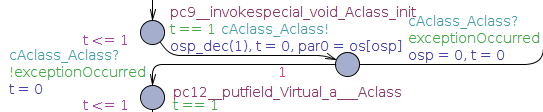
\includegraphics[width=\textwidth]{invokespecial.png}
  \caption{Invokespecial Instruction.}
\end{subfigure}
\hspace{10px}
\begin{subfigure}{.25\textwidth}
  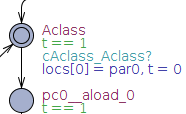
\includegraphics[width=\textwidth]{initloc.png}
  \caption{Initial Location.}
\end{subfigure}
\caption{Java bytecode and corresponding UPPAAL model.}
\label{fig:invokespecial}
\end{figure}


\subsubsection{Virtual Methods}
Virtual methods are similar to static methods in regards to representation in the method template for caller and callee, but instead of handling control directly to callee method templates, a template responsible for resolving the virtual call is inserted for this purpose.
\cref{fig:invokevirtual} is the resolver template generated for the code in \cref{lst:virtual}, there is a total of three virtual methods in this sample and the resolver has a waiting location for each.\\\\
Every class is mapped to an integer $clID$ and an array, $classHierarchy$, represents the class hierarchy of the program. The initial location \UPP{Invoke} waits for a synchronisation, after which the location \UPP{Resolver} has an outgoing edge for every possibility, in this sample that is five. There are essentially always three distinct possibilities 

\begin{itemize}
\item There are no methods and no super where $clID == 0$.
\item There is a method matching the class and method signature. In this case, call the method.
\item There are no methods but there is a super class, then assign $clID = classHierarchy[clID]$ and try again.
\end{itemize}

This is based on $methodLookup$ from the \texttt{INVOKEVIRTUAL} semantics from \cref{app:invokevirtual}. The usage of template for resolving method calls have similar limitation as representing a template as a method, discussed in \cref{sec:programConversion}. It pose a problem when calling virtual methods from within a virtual method, but it can be handling by instantiating a instant of the lookup template for each virtual method, this however might scale poorly.

 
\begin{figure}[H]
\centering
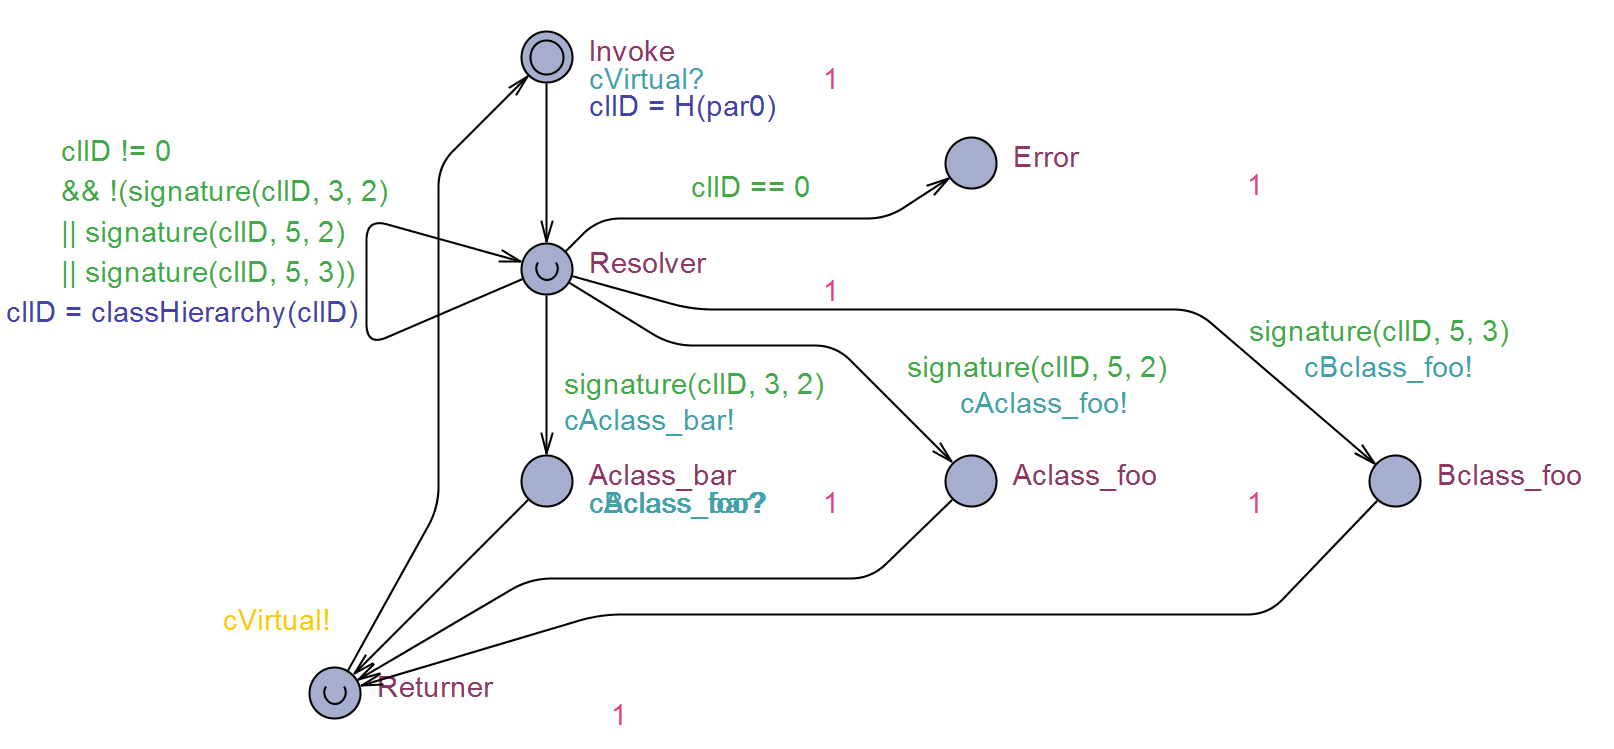
\includegraphics[width=\textwidth]{invoke.PNG}
\caption{Invokevirtual.}
\label{fig:invokevirtual}
\end{figure}

\subsubsection{Exceptions}
\label{sec:exceptions}
Exceptions are handled by \texttt{try catch} blocks which does not have a corresponding bytecode instruction, instead they are defined at the end of a method as seen in \cref{lst:exception}, \texttt{0, 8, 11} represents the corresponding program counters (pc).
When exceptions are thrown by the \texttt{athrow} instruction, there are two outcomes, either there is some exception handling covering the \texttt{athrow} defined in the current method, in which case the execution continues from the \texttt{catch start} pc. 
If there is no exception handling covering the \texttt{athrow}, the top stack frame will be poped and the process repeat, no handling and the new top frame is poped. On \jc an unhandled exception by the applet can be used to indicate an error such as \textit{no access}.\\

\noindent The \UPP{athrow} location have an edge to a new location, this is required to set a flag for \textit{exception occurred} before synchronising passing control back to the caller. In \cref{fig:uppaal3}a the caller is shown and if the \textit{exception occurred} flag is set when amusing control, it will follow the edge to, in this example, the initial instruction. It is also possible for the \UPP{athrow} location to have an edge to a \texttt{catch} pc instruction, depending on the exception definition.




\begin{lstlisting}[caption={Invokespecial Bytecode generated by Sawja.},numbers=none,label={lst:exception}]
....
try start: 0; try end: 8: catch start: 11; catched type: java.lang.Exception.
\end{lstlisting}






\section{Fault Modelling}
We focus on three faults: program counter, data fault and static instruction fault where program counter and data fault is considered transient faults and static instruction fault is considered a persistent fault as described in \cref{sec:faultsce}.

\subsection{Program Counter Fault}
\ch{we should also show how we have modelled a fault in the heap/stack}
To model a single bit flip occurring in the program's execution a special fault template is introduced, illustrated in \cref{fig:faultTime}. The template selects a random value between $0$ and the maximum possible global clock value, which represents when in the programs execution a fault happens. The random value is assigned to a global variable in the UPPAAL system.\\\\
Every instruction in the Java bytecode is represented by a location, and has an associated program counter. There are edges from each location going to the locations which can be reached if one bit is flipped in the program counter. These edges have guards which check whether the time the fault is injected, corresponds to the global clock at the time the model simulation is at that particular edge. If it is, the guard will allow the edge to be traversed. There are no fault edges going back to the added locations described in \cref{subsubsec:method}, since these are not a part of the original program and therefore do not have an associated program counter.
\begin{figure}[H]
\centering
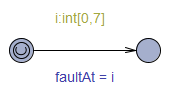
\includegraphics{figures/fault.PNG}
\caption{The UPPAAL template which selects when to perform a bit flip in the program counter}
\label{fig:faultTime}
\end{figure}\ch{update figure to use fault at between 0 and global clock}

\subsection{Data Faults}
% locals and opstack
To introduce data fault for the operand stack a special template selects when a fault should be introduced into the operand stack. This happens in the same way as in the \textit{program counter} fault described earlier, illustrated in \cref{fig:faultTime}. The selected value is between $0$ and the maximum possible runtime of the program. \cref{fig:opstackFlip} shows how a method called \texttt{getTriesRemaining}, in which a bit flip in the operand stack occurs. Edges going back to the locations \texttt{pc0\_iconst\_2} and \texttt{pc0\_iconst\_2} are where the faults are introduced, these are added by the solution and are not a part of an unaltered model of a program. The edges have a guard, $faultTime \leq globalClock$, determined by the special template, which only allows a fault to happen if the program execution has executed for a certain amount of time. The fault itself is introduced by the update $os\lbrack osPos \rbrack\:\hat{}= 1 \ll osBitPos$, which flips bit \UPP{osBitPos} of value \UPP{osPos} in the operand stack\ch{ref to description of how we represent operand stack here?}. \UPP{osBitPos} is a random value between $0$ and $7$, which denotes which bit should be flipped. \UPP{osPos} is a random value between $0$ and the maximum size of the operand stack. After a fault has been introduced, the variable \UPP{faultTime} is set to a value higher than the maximum value of the global clock, to ensure only one fault happens per simulation.\\\\
Our approaches to modelling faults in the operand stack, heap and local variables are similar and only one of them is therefore described.\ch{is this enough or should we tell more about how the heap modelling works?}
% % % % %
\begin{figure}[H]
\centering
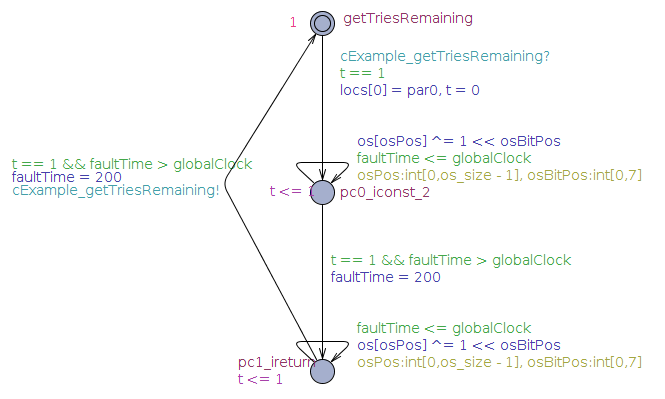
\includegraphics[width=\textwidth]{figures/reportExamples/opstackRewrite.png}
\caption{The UPPAAL model af a method where a bit flip occurs in the operand stack.}
\label{fig:opstackFlip}
\end{figure}
\subsection{Static Instruction Fault}
Instruction faults are modelled by first assigning each edge of all templates a unique identifier. A special template then selects a random value in the range of $0$ and the greatest identifier in the modelled program. It is not time-dependent, i.e. it does not rely on a clock the \textit{operand stack} fault described earlier. A fault will only happen once since only one identifier is selected, and only when the simulation reaches the instruction chosen by the special template. This is enforced using guards which compares the selected identifier with the current edge's. During the generation of the model, the solution has calculated all instructions, an instruction can be changed to by a bit flip in their binary encoding. Additional edges are then inserted to perform the actions of the altered instructions. For example, the \texttt{ifeq} instruction, which can be bit flipped to \texttt{goto}, would cause an extra edge representing the "yes" branch to be created to the destination location of the original "yes" branch. The new edge is different from the two original edges by always being enabled, thus causing a simulation to always perform a jump regardless of the result of an \texttt{ifeq} comparison.

\section{Proposed Solution}
this is a test

%\begin{figure}[H]
%\centering
%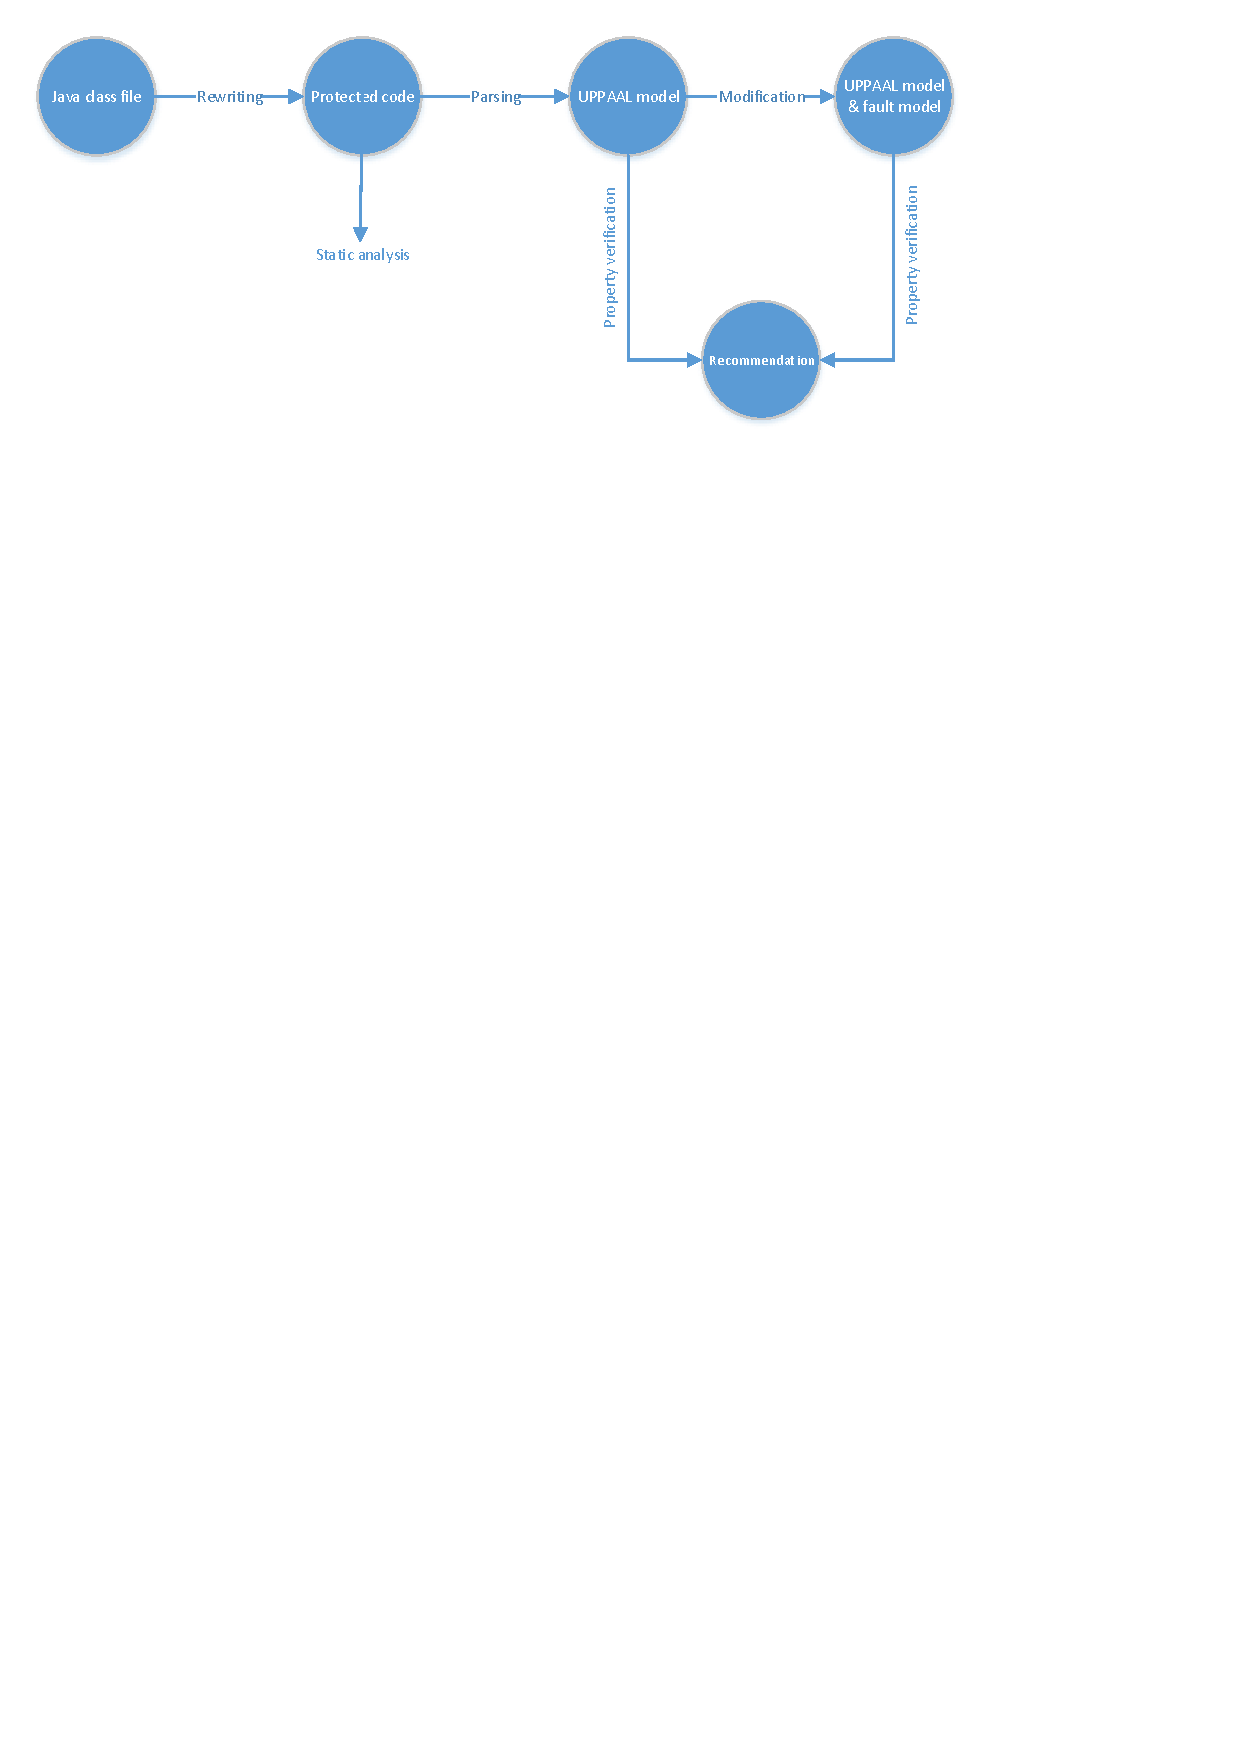
\includepdf[pages={1}, scale=0.8]{workflow.pdf}
%\caption{Workflow}
%\end{figure}
